\documentclass{beamer}
\usepackage[english]{babel}
\usepackage{tikz}
\usepackage{aeguill}
\usepackage{amsmath}
\usepackage{blkarray}
\usepackage{hyperref}
\usepackage{color}
\usepackage{pgf, pgffor}
\usepackage{listings}
\usepackage{xcolor}
\usepackage{etoolbox}
\usepackage{tcolorbox}
\usepackage{float}


\date{10. Juli 1732}

\usetheme{Boadilla}
%\usecolortheme{beaver}
\usecolortheme{seahorse}

\title{Sensor technology}
\author{Arthur, Roland, Thomas}


%
% !!!!!!!!!!!!!!!!!!!!!!!!!!!!!!!!!!!!!!!!!!!!!
%   Bitte wieder in einzenle files aufteilen, 
%   dann sparen wir uns die tollen merge conflicts. :-)
% !!!!!!!!!!!!!!!!!!!!!!!!!!!!!!!!!!!!!!!!!!!!!
%


\begin{document}
\begin{frame}
    \titlepage
\end{frame}

\begin{frame}
    \frametitle{Welches Thema haben wir bearbeitet?}

    \begin{itemize}
        \item Weniger Strom und so
              \begin{itemize}
                  \item Implementierung
                  \item Tests
              \end{itemize}
    \end{itemize}
\end{frame}

\begin{frame}
    \frametitle{Wie lauteten unsere Forschungsfragen?}

    \begin{itemize}
        \item Ist die Erde rund?
        \item Warum hat ein Dreieck genau drei Ecken?
        \item Warum sollen wir das Rad nicht neu erfinden?
    \end{itemize}
\end{frame}

\begin{frame}
    \frametitle{How to side by side?}
    \framesubtitle{Fancy subtitle}

    \begin{columns}
        \begin{column}{0.5\textwidth}
            \begin{itemize}
                \item A
                      \begin{itemize}
                          \item A1
                          \item A2
                      \end{itemize}
            \end{itemize}
        \end{column}
        \begin{column}{0.5\textwidth}
            \textit{Lala}
        \end{column}
    \end{columns}
\end{frame}

\begin{frame}
    \frametitle{Experimental Setup}
	\begin{minipage}[t]{0.60 \textwidth}
		\begin{figure}[H]
			\centering
			\vspace{20pt}
			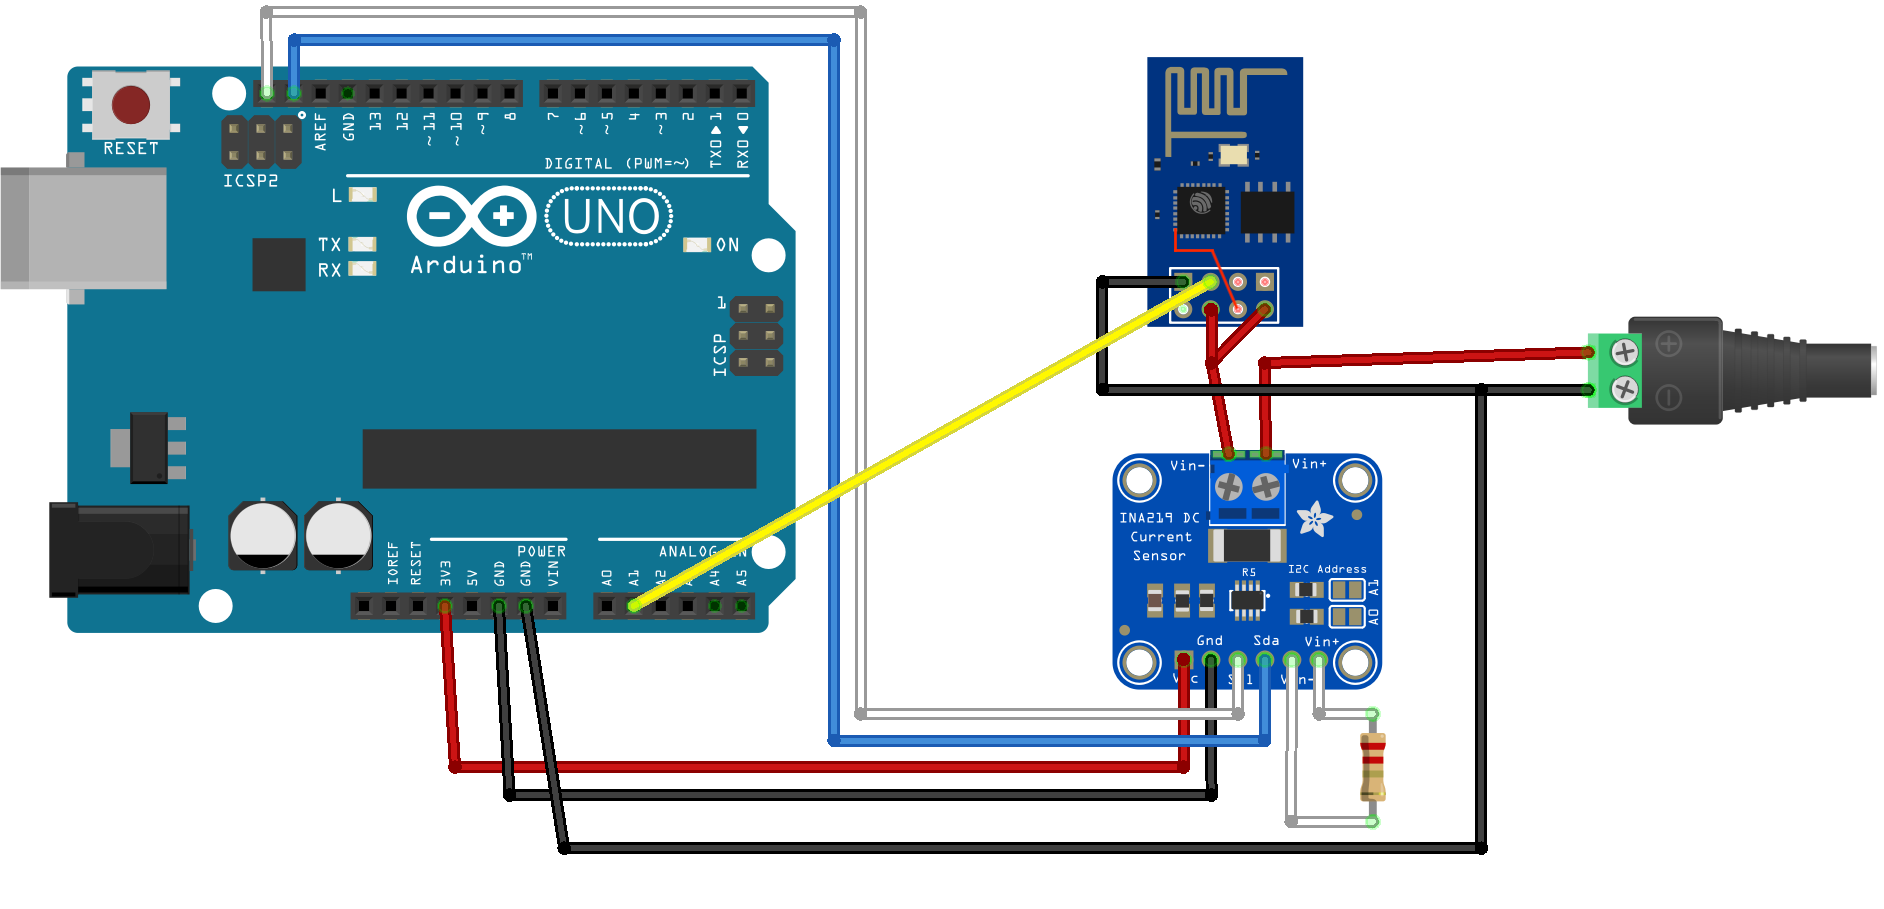
\includegraphics[width = 1.4 \linewidth]{fig/experimental_setup.png}
		\end{figure}
	\end{minipage}
	\begin{minipage}[t]{0.30 \textwidth}
		\begin{itemize} 
			\item ESP8266-01s
			\item Adafruit INA219
			\item $2.2\Omega$ Resistor
			\item Arduino UNO
		\end{itemize}
	\end{minipage}
\end{frame}


\begin{frame}
    \frametitle{Unterschied zwischen DHCP und einer statischen IP?}
    \framesubtitle{Im Hinblick auf den Energieverbrauch}

    \begin{columns}
        \begin{column}{0.5\textwidth}
            \begin{itemize}
                \item DHCP
                      \begin{itemize}
                          \item DHCP Server
                          \item Dynamische Zuweisung von IP Adressen
                          \item Lease time
                      \end{itemize}
            \end{itemize}
        \end{column}
        \begin{column}{0.5\textwidth}
            \begin{itemize}
                \item Statische IP-Adresse
                      \begin{itemize}
                          \item IP Adresse bleibt statisch
                          \item Vergewissern, dass Adresse verfügbar
                      \end{itemize}
            \end{itemize}
        \end{column}
    \end{columns}
\end{frame}

\begin{frame}
    \frametitle{DHCP}
    \begin{columns}
        \begin{column}{0.5\textwidth}
            \begin{itemize}
                \item 4 Schritte notwendig
                \item IP Adresse nur "geliehen"
                \item Lease time-Erneuerung

            \end{itemize}
        \end{column}
        \begin{column}{0.5\textwidth}
            \begin{figure}
                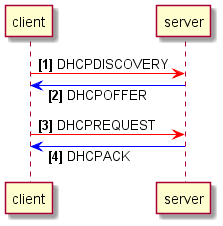
\includegraphics[scale=0.7]{../paper/fig/sequence_DHCP_connection.png}
            \end{figure}
        \end{column}
    \end{columns}
\end{frame}

\begin{frame}
    \frametitle{Experimentdurchlauf: DHCP}
    \begin{figure}
        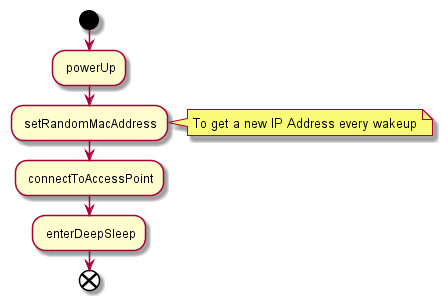
\includegraphics[scale=0.6]{../paper/fig/sequence_DHCP.png}
    \end{figure}
\end{frame}

\begin{frame}
    \frametitle{Experimentdurchlauf: Statische IP}
    \begin{figure}
        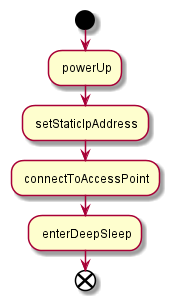
\includegraphics[scale=0.6]{../paper/fig/sequence_static_ip.png}
    \end{figure}
\end{frame}

\begin{frame}
    \frametitle{Messergebnisse: DHCP}
    \begin{columns}
        \begin{column}{0.35\textwidth}
            \begin{itemize}
                \item $\overline{Dauer}$: $\approx5.5s$
                \item $\overline{Verbrauch}$: $\approx0.35As$
            \end{itemize}
        \end{column}
        \begin{column}{0.65\textwidth}
            \begin{figure}
                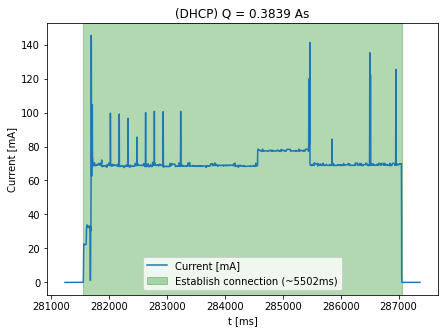
\includegraphics[scale=0.5]{../paper/fig/dhcp.png}
            \end{figure}
        \end{column}
    \end{columns}
\end{frame}

\begin{frame}
    \frametitle{Messergebnisse: Statische IP}
    \begin{columns}
        \begin{column}{0.35\textwidth}
            \begin{itemize}
                \item $\overline{Dauer}$: $\approx4.0s$
                \item $\overline{Verbrauch}$: $\approx0.28As$
            \end{itemize}
        \end{column}
        \begin{column}{0.65\textwidth}
            \begin{figure}
                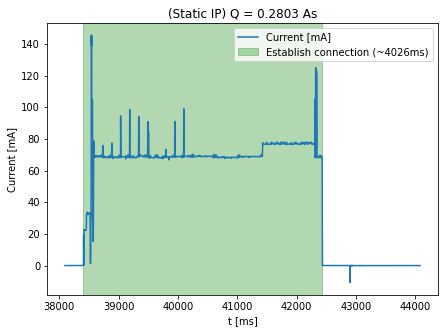
\includegraphics[scale=0.5]{../paper/fig/static_ip.png}
            \end{figure}
        \end{column}
    \end{columns}
\end{frame}

\begin{frame}
    \frametitle{Zusammenfassung}

    \begin{itemize}
        \item Verwenden einer statischen IP verbraucht $\approx 20.5\%$ weniger Strom
        \item Verbrauch beim Verwenden von DHCP abhängig von der Lease time
        \item Verbindungsaufbau über DHCP braucht $\approx 1.5s$ länger
    \end{itemize}


\end{frame}




    \subsection{Sleep modes}
Sleep modes are a very common way to improve the energy efficiency of micro controllers.
The basic idea is to reduce the power consumption by disabling unused modules in the chip and only power them up when they are needed.
In the case of the ESP8266, the vendor provides three different sleep modes. 
Table \ref{tab_sleep_modes} summarises the capabilities and typical current consumptions of the available sleep modes.
\cite{mesquita_assessing_2018}

\begin{table}[htbp]
\caption{ESP8266 sleep modes}
\begin{center}
\begin{tabular}{|c|c|c|c|}
\hline
\textbf{Module}&\textbf{Modem sleep}&\textbf{Light sleep}&\textbf{Deep sleep}\\
\hline
\textbf{WiFi} & OFF & OFF & OFF\\
\textbf{AP association} & Connected & Connected & Disconnected\\
\textbf{System clock} & ON & OFF & OFF\\
\textbf{RTC} & ON & ON & ON\\
\textbf{CPU} & ON & Pending & OFF\\
\hline
\textbf{Substrate current} & $15mA$ & $0.4mA$ & $20\mu A$\\
\hline
\end{tabular}
\label{tab_sleep_modes}
\end{center}
\end{table}

\subsubsection{Modem sleep} \label{sec:modem_sleep}
Modem sleep is the default sleep mode of the ESP8266 and is recommended for applications that require a real time CPU control. \cite{mesquita_assessing_2018}
By enabling the modem sleep, the ESP8266 will turn off the WiFi modem between the DTIM beacons. 
This improves the power consumption of the system and has the advantage that the system stays connected to the AP.\\
A typical use case is a WiFi controlled light bulb that provides real time light control.\cite{espressif_inc_esp8266_2016}

\subsubsection{Light sleep} \label{sec:light_sleep}
The light sleep mode is similar to the modem sleep mode with the additional improvement that the internal clock is powered off and the CPU is suspended when there are no tasks to execute.\\
According to the datasheet \cite{espressif_inc_esp8266_2016}, it takes less than $3ms$ to switch back into modem sleep mode.\\
This mode can be used when the application needs to stay connected to the access point 
and needs to responde to incoming data. The CPU is powered off when no data receives.

\subsubsection{Deep sleep} \label{sec:deep_sleep}
For ultra low power applications, the ESP8266 provides a deep sleep mode.
In this mode are all modules disabled except the real time clock (RTC) which can be used to wake up the controller periodically.
When the controller is in the deep sleep mode, it can only be woken up by applying a pulse to the RST pin.
This pulse can either be generated by an external device like a motion sensor or by the built in RTC module.\\
Another usefull feature is the RTC memory. This kind of memory makes it possible to store data over deep sleep cycles.
It losses the stored data only when the controller is disconnected from the power supply.
A possible use case is, to collect multiple measurement samples over time and send them out in a single package.\\
Deep sleep can be used for ultra low power applications that can be idle most of the time. 
However, there is the limitation that the system is not reachable from the outside at all times. \cite{espressif_inc_esp8266_2016}

\subsection{UDP and TCP}
\label{udptcp:sci}
\subsubsection{TCP}
\label{tcp:sci}
Transmission Control Protocol is a connection-oriented network protocol
for sending data over a network.
This means that TCP waits until a connection is established and
then starts transmitting data\cite{postel1981transmission}.
TCP guaratees that data is transmitted to recipiend
in the correct order and without corrupt segments.
As a downside, this creates an enormous overhead compared
to other network protocols\cite{singh2014survey}\newline.
\subsubsection{UDP}
\label{udp:sci}
User Datagram Protocol is a connectionless network protocol
\cite{postel1980user}.
This protocol has no error handling or recovery options for
 the transmission and sends the data continuously.
It is not necessary for the sender that the client 
receives the data.
Compared to TCP, it allows less overhead when transferring data
\cite{singh2014survey}.

\end{document}